% CREATED BY DAVID FRISK, 2016
\chapter{Revised Materials}
\vspace{-1cm}
\section{Links to teaching materials}
\vspace{-0.5cm}
\bgroup
\def\arraystretch{1.5}
\begin{table}[H]
\begin{adjustwidth}{-2cm}{}
\centering
\caption{Summary of all revisions in this study.}
  \begin{tabular}{p{4.5cm}p{7cm}p{6.5cm}} \hline\hline
  \textbf{Name of material} & \textbf{URL to original} & \textbf{URL to revised version} \\ \hline
  Konsten att bestämma arean & \url{https://kleindagarna.se/app/uploads/13kleinlektionAnalys.pdf} & \url{https://github.com/Niwsters/teaching-materials-thesis/raw/master/revisions/material_bestamma_arean_revision.odt} \\ \hline
  Den dolda och tvetydiga matematiken & \url{https://kleindagarna.se/app/uploads/13kleinlektionalge.pdf} & \url{https://github.com/Niwsters/teaching-materials-thesis/raw/master/revisions/material_tvetydiga_matematiken_revision.odt} \\ \hline
  Vad ska lotten kosta? & \href{https://kleindagarna.se/app/uploads/Kleindagar-augusti-2017-lektionsutkast-Grupp-1-Finansmatematik-20170820.pdf}{\nolinkurl{https://kleindagarna.se/app/uploads/Kleindagar-augusti-2017-}} \href{https://kleindagarna.se/app/uploads/Kleindagar-augusti-2017-lektionsutkast-Grupp-1-Finansmatematik-20170820.pdf}{\nolinkurl{lektionsutkast-Grupp-1-}} \href{https://kleindagarna.se/app/uploads/Kleindagar-augusti-2017-lektionsutkast-Grupp-1-Finansmatematik-20170820.pdf}{\nolinkurl{Finansmatematik-20170820.pdf}}& \url{https://github.com/Niwsters/teaching-materials-thesis/raw/master/revisions/material_lotteri_revision.odt}\\ \hline
  Mönster och talföljder - Pascals triangel ur slantsingling & \href{https://kleindagarna.se/app/uploads/Kleinlektion-augusti-2017-rev-vers-170821.pdf}{\nolinkurl{https://kleindagarna.se/app/uploads/Kleinlektion-augusti-2017-}} \href{https://kleindagarna.se/app/uploads/Kleinlektion-augusti-2017-rev-vers-170821.pdf}{\nolinkurl{rev-vers-170821.pdf}} & \url{https://github.com/Niwsters/teaching-materials-thesis/blob/master/revisions/material_pascals_triangel_revision.odt} \\ \hline
  Nätverk - insamling av data & \href{http://kleindagarna.se/app/uploads/Kleinlektion-grupplektion-Natverk.pdf}{\nolinkurl{http://kleindagarna.se/app/uploads/Kleinlektion-grupplektion-}} \href{http://kleindagarna.se/app/uploads/Kleinlektion-grupplektion-Natverk.pdf}{\nolinkurl{Natverk.pdf}} & \url{https://github.com/Niwsters/teaching-materials-thesis/raw/master/revisions/material_natverk_revision.pptx}\\ \hline
\end{tabular}
\label{app:revisions}
\end{adjustwidth}
\end{table}
\egroup
\vspace{-0.5cm}
Here is another valuable link pointing to a list of all materials, including Swedish descriptions and more  (last updated 2018-08-22):\\
\url{https://niwsters.github.io/teaching-materials-thesis/}


\newpage

\section{Revised Kleinmaterial: Nätverk}
\label{app:case1}
\begin{comment}
            \begin{figure}[H]
            \begin{adjustwidth}{-2.5cm}{}
                    \begin{tabular}{@{}c@{\hspace{.1cm}}c@{}}
                        \subsubsection*{Presentation slides} &
                        \subsubsection*{Teacher notes}\\
                        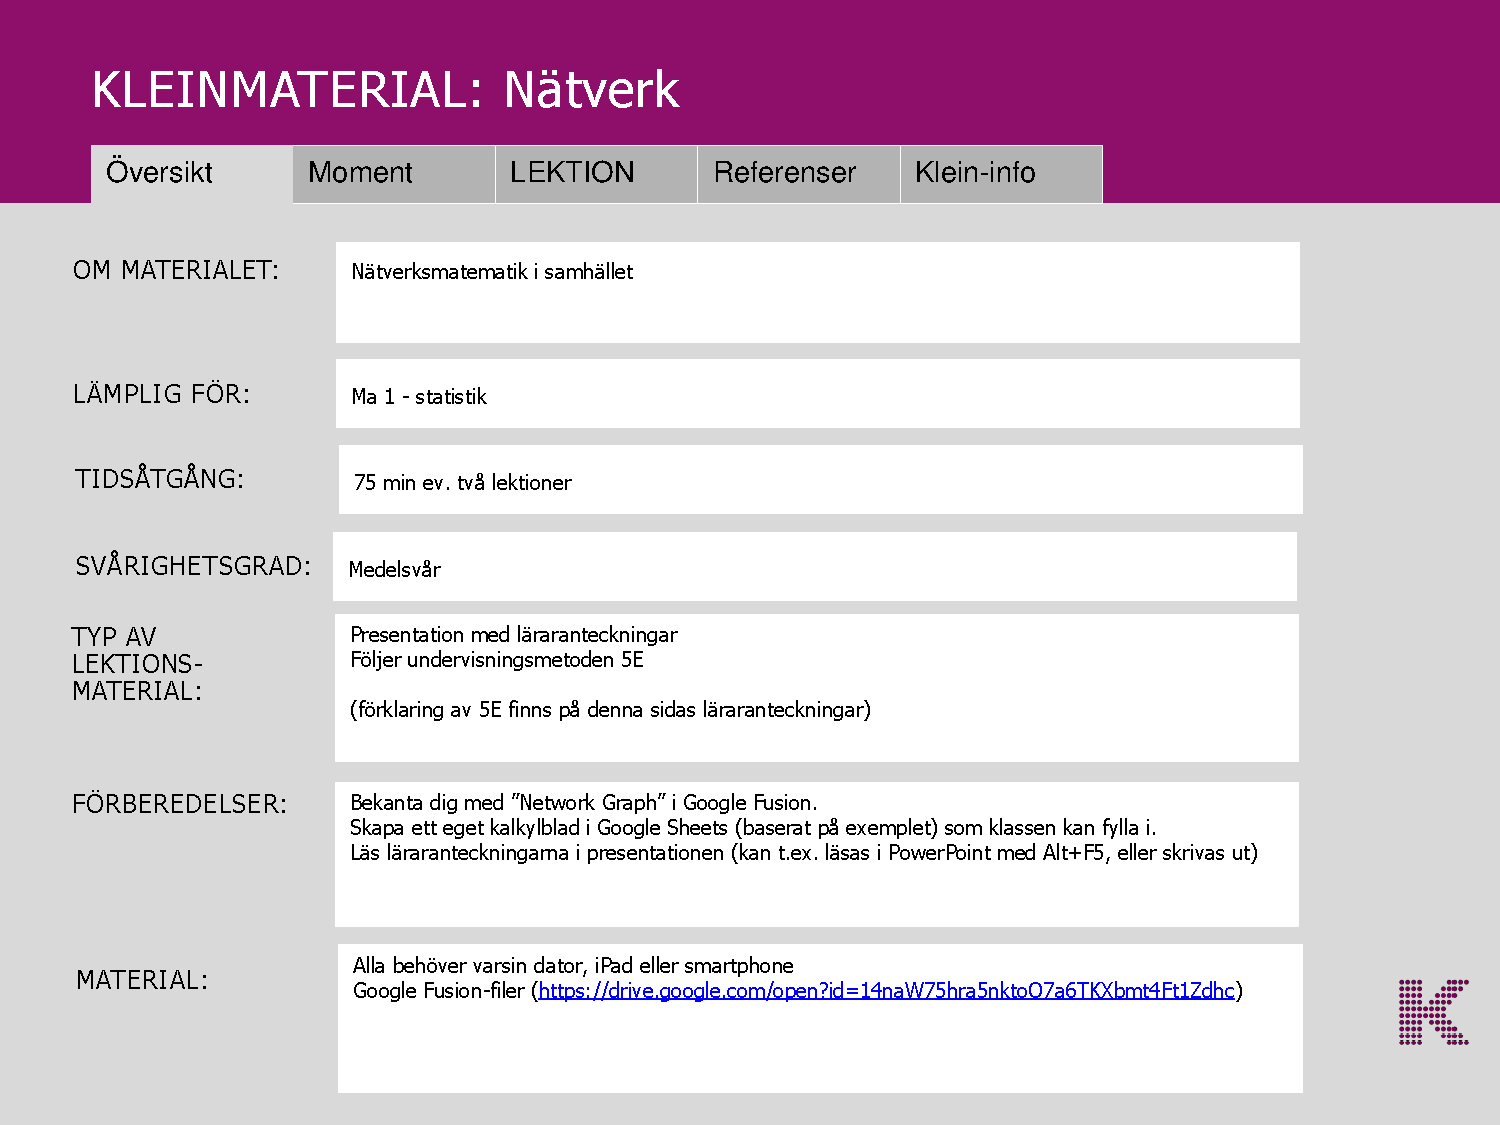
\includegraphics[page=1,width=0.68\textwidth]{pdf/natverk} &
                        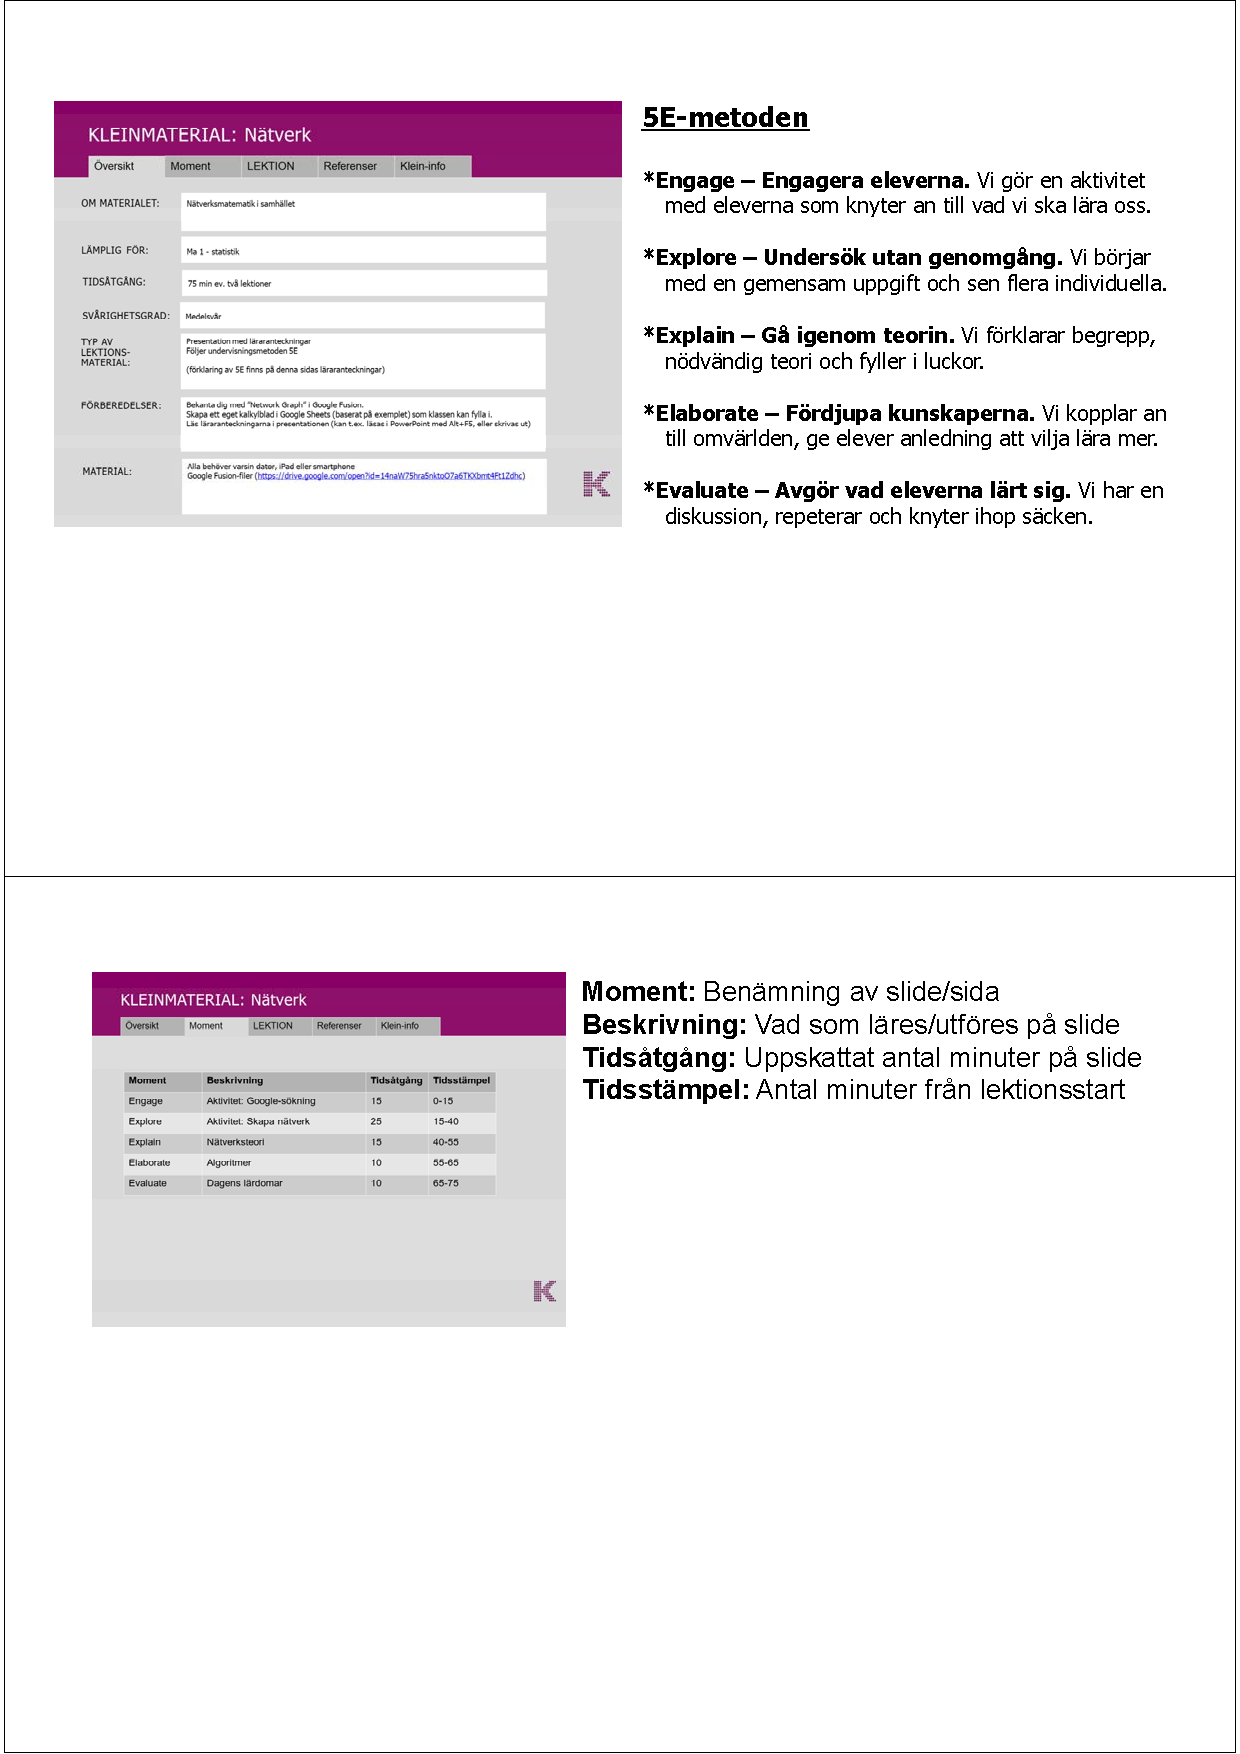
\includegraphics[page=1,width=0.68\textwidth]{pdf/notes}\\
                        \includegraphics[page=2,width=0.68\textwidth]{pdf/natverk} &
                        \includegraphics[page=2,width=0.68\textwidth]{pdf/notes} \\
                    \end{tabular}
            \end{adjustwidth}
            \end{figure}
            
            \newpage
            \begin{figure}[H]
            \begin{adjustwidth}{-2.5cm}{}
                    \begin{tabular}{@{}c@{\hspace{.1cm}}c@{}}
                        \includegraphics[page=3,width=0.68\textwidth]{pdf/natverk} &
                        \includegraphics[page=3,width=0.68\textwidth]{pdf/notes}\\
                        \includegraphics[page=4,width=0.68\textwidth]{pdf/natverk} &
                        \includegraphics[page=4,width=0.68\textwidth]{pdf/notes} \\
                        \includegraphics[page=5,width=0.68\textwidth]{pdf/natverk} &
                        \includegraphics[page=5,width=0.68\textwidth]{pdf/notes} \\
                    \end{tabular}
            \end{adjustwidth}
            \end{figure}
            
            \newpage
            \begin{figure}[H]
            \begin{adjustwidth}{-2.5cm}{}
                    \begin{tabular}{@{}c@{\hspace{.1cm}}c@{}}
                        \includegraphics[page=6,width=0.68\textwidth]{pdf/natverk} &
                        \includegraphics[page=6,width=0.68\textwidth]{pdf/notes}\\
                        \includegraphics[page=7,width=0.68\textwidth]{pdf/natverk} &
                        \includegraphics[page=7,width=0.68\textwidth]{pdf/notes} \\
                        \includegraphics[page=8,width=0.68\textwidth]{pdf/natverk} &
                        \includegraphics[page=8,width=0.68\textwidth]{pdf/notes} \\
                    \end{tabular}
            \end{adjustwidth}
            \end{figure}
            
            \newpage
            \begin{figure}[H]
            \begin{adjustwidth}{-2.5cm}{}
                    \begin{tabular}{@{}c@{\hspace{.1cm}}c@{}}
                        \frame{\includegraphics[page=9,width=0.68\textwidth]{pdf/natverk}} &
                        \frame{\includegraphics[page=9,width=0.68\textwidth]{pdf/notes}}\\
                        \frame{\includegraphics[page=10,width=0.68\textwidth]{pdf/natverk}} &
                        \frame{\includegraphics[page=10,width=0.68\textwidth]{pdf/notes}} \\
                    \end{tabular}
            \end{adjustwidth}
            \end{figure}
\end{comment}
           
\begin{figure}[H]
%\begin{adjustwidth}{-2.5cm}{}
    \begin{tabular}{l}%{@{}c@{\hspace{.1cm}}c@{}}
       % \subsubsection*{Presentation slides and teacher notes}\\
            Presentation slide 1 of 10\\
            \frame{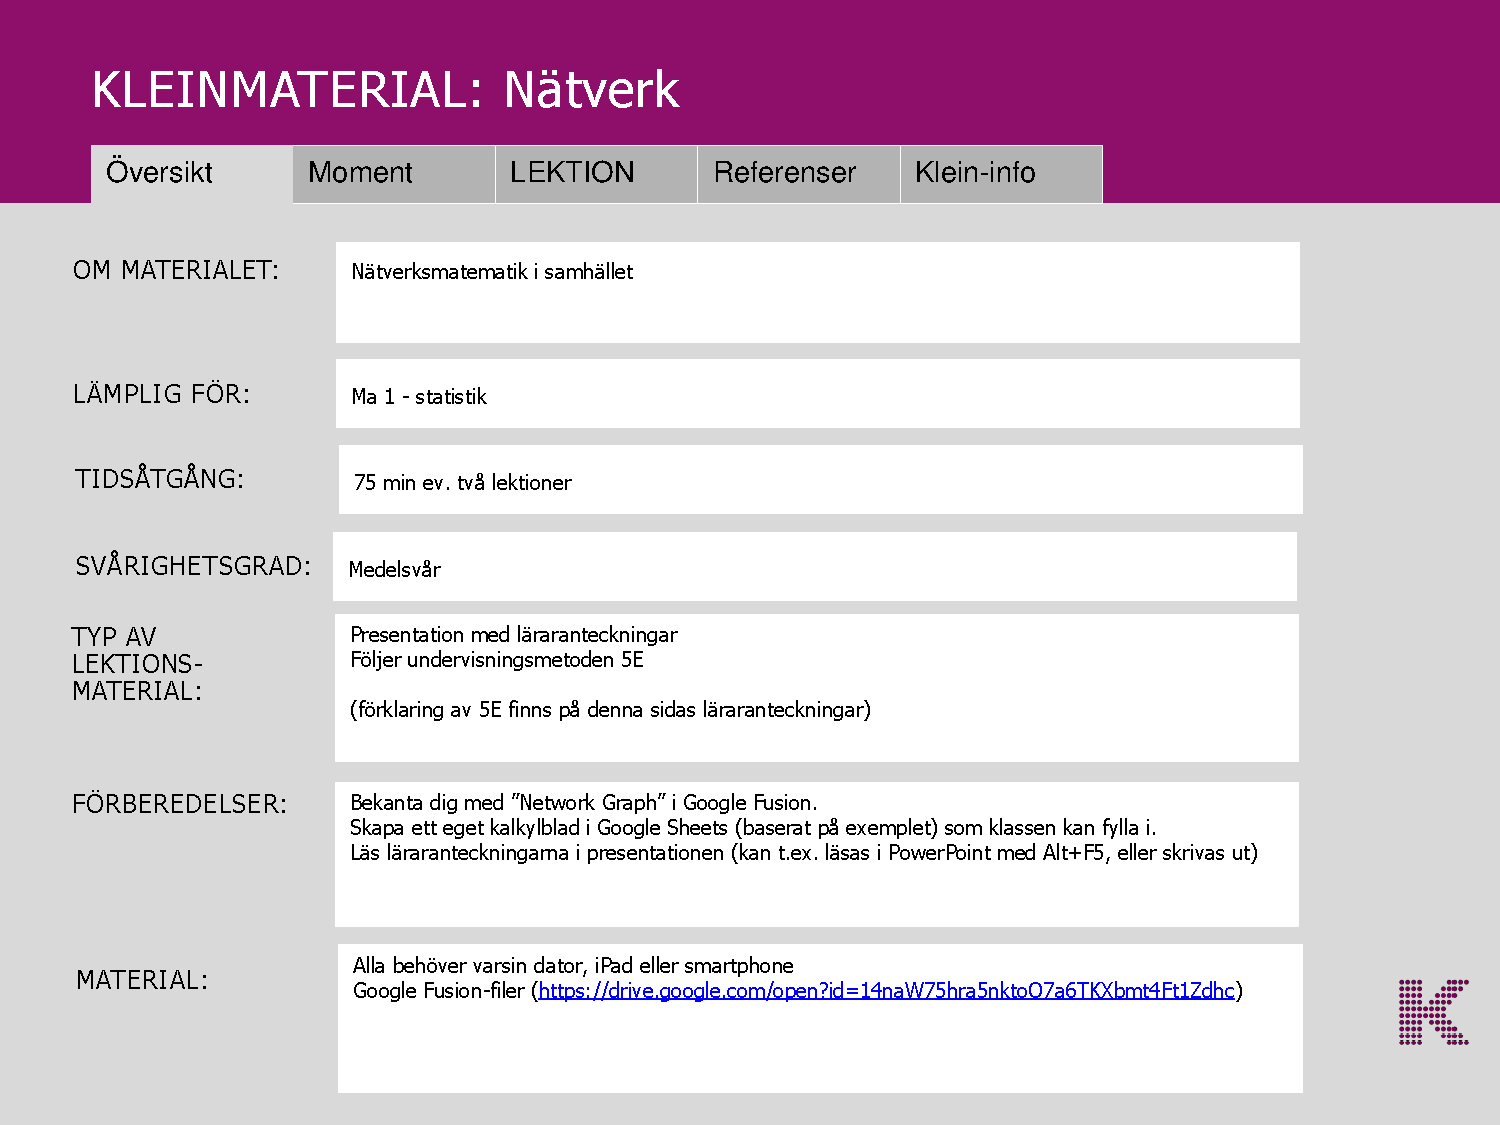
\includegraphics[page=1,width=1\textwidth]{pdf/natverk}}\\
            \\
            Teacher notes slide 1 of 10\\
            \frame{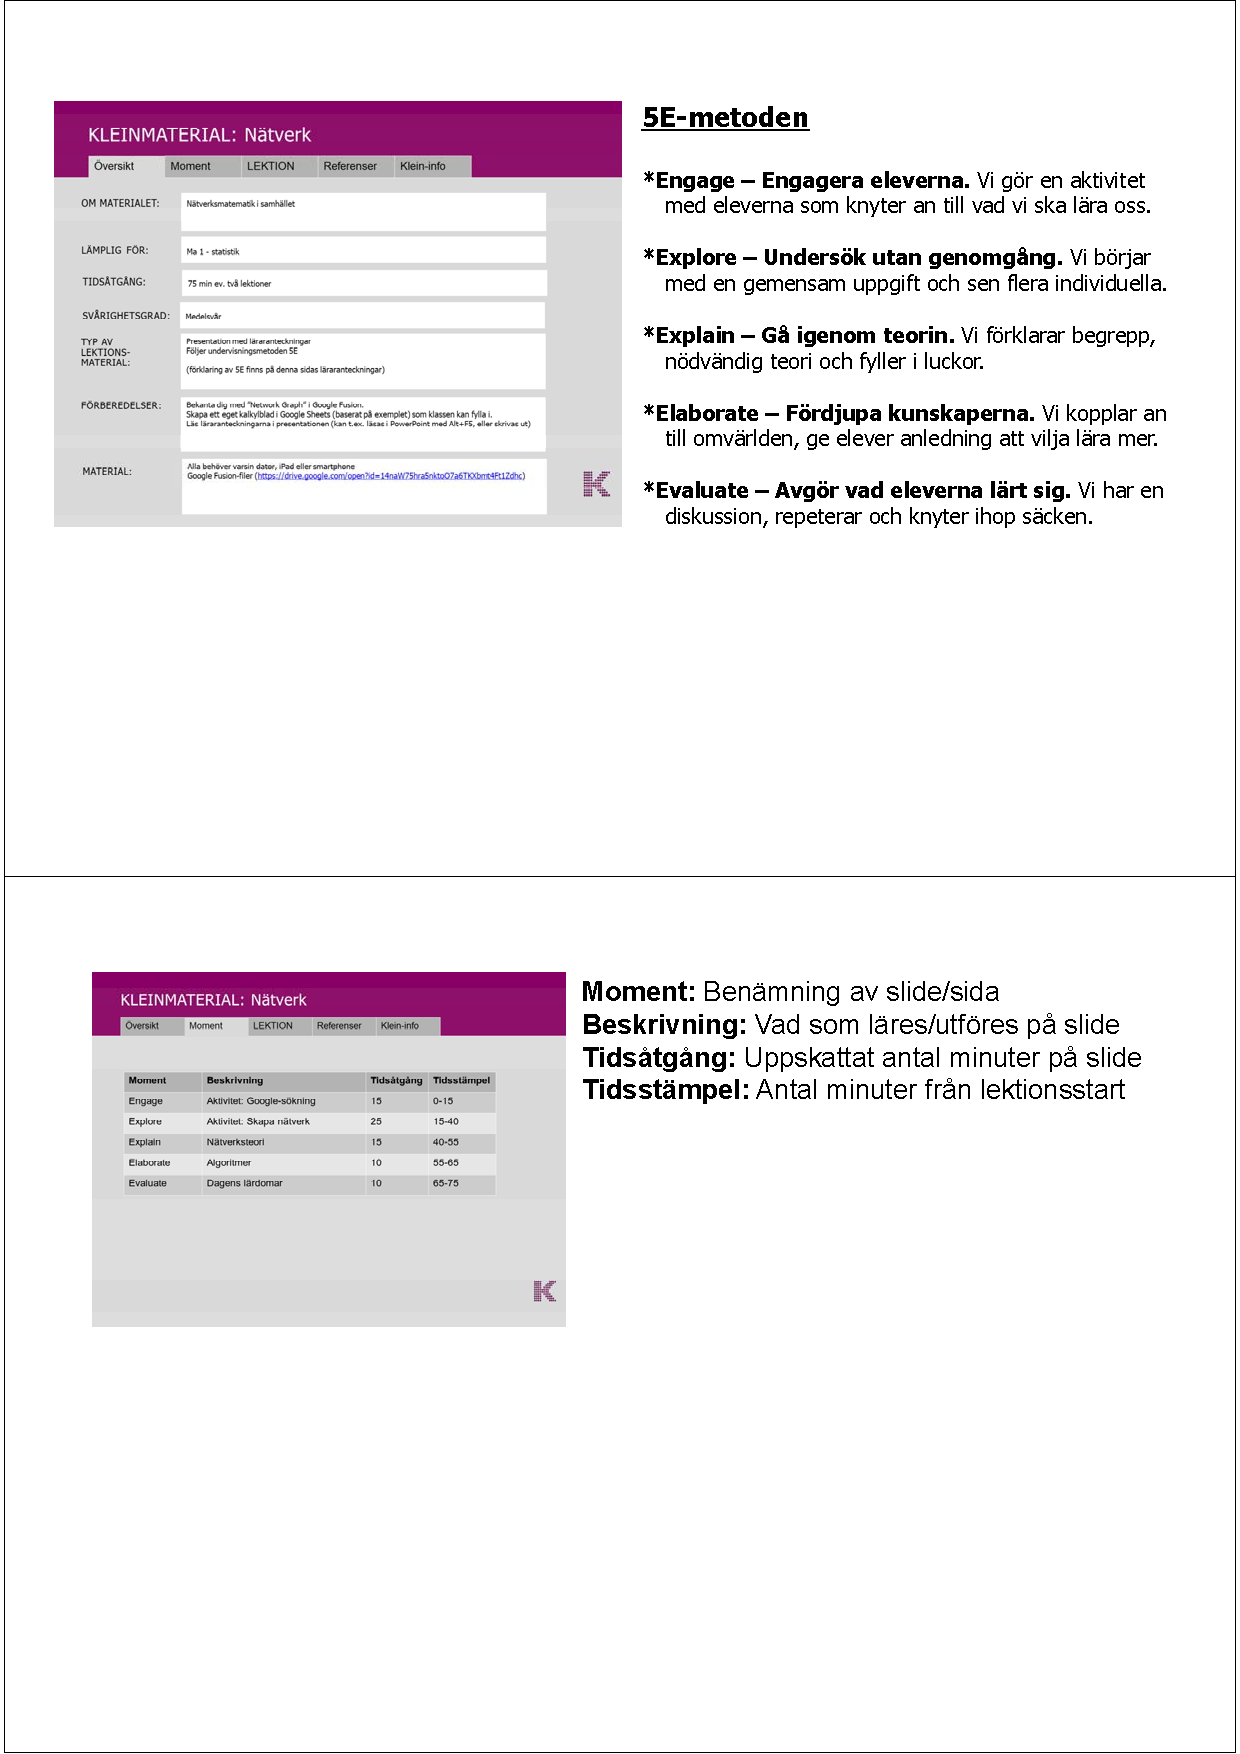
\includegraphics[trim={0 3.5cm 0 0},clip,page=1,width=1\textwidth]{pdf/notes}}\\
        \end{tabular}
%\end{adjustwidth}
\end{figure}
            
\newcommand{\slidenr}{2 }
\newpage
\begin{figure}[H]
%\begin{adjustwidth}{-2.5cm}{}
    \begin{tabular}{l}%{@{}c@{\hspace{.1cm}}c@{}}
            Presentation slide \slidenr of 10\\
            \frame{\includegraphics[page=\slidenr,width=1\textwidth]{pdf/natverk}}\\
            \\
            Teacher notes slide \slidenr of 10\\
            \frame{\includegraphics[trim={0 0cm 0 0},clip,page=\slidenr,width=1\textwidth]{pdf/notes}}\\
        \end{tabular}
%\end{adjustwidth}
\end{figure}

\renewcommand{\slidenr}{3 }
\newpage
\begin{figure}[H]
%\begin{adjustwidth}{-2.5cm}{}
    \begin{tabular}{l}%{@{}c@{\hspace{.1cm}}c@{}}
            Presentation slide \slidenr of 10\\
            \frame{\includegraphics[page=\slidenr,width=1\textwidth]{pdf/natverk}}\\
            \\
            Teacher notes slide \slidenr of 10\\
            \frame{\includegraphics[trim={0 0cm 0 0},clip,page=\slidenr,width=1\textwidth]{pdf/notes}}\\
        \end{tabular}
%\end{adjustwidth}
\end{figure}

\renewcommand{\slidenr}{4 }
\newpage
\begin{figure}[H]
%\begin{adjustwidth}{-2.5cm}{}
    \begin{tabular}{l}%{@{}c@{\hspace{.1cm}}c@{}}
            Presentation slide \slidenr of 10\\
            \frame{\includegraphics[page=\slidenr,width=1\textwidth]{pdf/natverk}}\\
            \\
            Teacher notes slide \slidenr of 10\\
            \frame{\includegraphics[trim={0 0cm 0 0},clip,page=\slidenr,width=1\textwidth]{pdf/notes}}\\
        \end{tabular}
%\end{adjustwidth}
\end{figure}

\renewcommand{\slidenr}{5 }
\newpage
\begin{figure}[H]
%\begin{adjustwidth}{-2.5cm}{}
    \begin{tabular}{l}%{@{}c@{\hspace{.1cm}}c@{}}
            Presentation slide \slidenr of 10\\
            \frame{\includegraphics[page=\slidenr,width=1\textwidth]{pdf/natverk}}\\
            \\
            Teacher notes slide \slidenr of 10\\
            \frame{\includegraphics[trim={0 0cm 0 0},clip,page=\slidenr,width=1\textwidth]{pdf/notes}}\\
        \end{tabular}
%\end{adjustwidth}
\end{figure}

\renewcommand{\slidenr}{6 }
\newpage
\begin{figure}[H]
%\begin{adjustwidth}{-2.5cm}{}
    \begin{tabular}{l}%{@{}c@{\hspace{.1cm}}c@{}}
            Presentation slide \slidenr of 10\\
            \frame{\includegraphics[page=\slidenr,width=1\textwidth]{pdf/natverk}}\\
            \\
            Teacher notes slide \slidenr of 10\\
            \frame{\includegraphics[trim={0 0cm 0 0},clip,page=\slidenr,width=1\textwidth]{pdf/notes}}\\
        \end{tabular}
%\end{adjustwidth}
\end{figure}

\renewcommand{\slidenr}{7 }
\newpage
\begin{figure}[H]
%\begin{adjustwidth}{-2.5cm}{}
    \begin{tabular}{l}%{@{}c@{\hspace{.1cm}}c@{}}
            Presentation slide \slidenr of 10\\
            \frame{\includegraphics[page=\slidenr,width=1\textwidth]{pdf/natverk}}\\
            \\
            Teacher notes slide \slidenr of 10\\
            \frame{\includegraphics[trim={0 0cm 0 0},clip,page=\slidenr,width=1\textwidth]{pdf/notes}}\\
        \end{tabular}
%\end{adjustwidth}
\end{figure}

\renewcommand{\slidenr}{8 }
\newpage
\begin{figure}[H]
%\begin{adjustwidth}{-2.5cm}{}
    \begin{tabular}{l}%{@{}c@{\hspace{.1cm}}c@{}}
            Presentation slide \slidenr of 10\\
            \frame{\includegraphics[page=\slidenr,width=1\textwidth]{pdf/natverk}}\\
            \\
            Teacher notes slide \slidenr of 10\\
            \frame{\includegraphics[trim={0 0cm 0 0},clip,page=\slidenr,width=1\textwidth]{pdf/notes}}\\
        \end{tabular}
%\end{adjustwidth}
\end{figure}

\renewcommand{\slidenr}{9 }
\newpage
\begin{figure}[H]
%\begin{adjustwidth}{-2.5cm}{}
    \begin{tabular}{l}%{@{}c@{\hspace{.1cm}}c@{}}
            Presentation slide \slidenr of 10\\
            \frame{\includegraphics[page=\slidenr,width=1\textwidth]{pdf/natverk}}\\
            \\
            Teacher notes slide \slidenr of 10\\
            \frame{\includegraphics[trim={0 0cm 0 0},clip,page=\slidenr,width=1\textwidth]{pdf/notes}}\\
        \end{tabular}
%\end{adjustwidth}
\end{figure}

\renewcommand{\slidenr}{10 }
\newpage
\begin{figure}[H]
%\begin{adjustwidth}{-2.5cm}{}
    \begin{tabular}{l}%{@{}c@{\hspace{.1cm}}c@{}}
            Presentation slide \slidenr of 10\\
            \frame{\includegraphics[page=\slidenr,width=1\textwidth]{pdf/natverk}}\\
            \\
            Teacher notes slide \slidenr of 10\\
            \frame{\includegraphics[trim={0 0cm 0 0},clip,page=\slidenr,width=1\textwidth]{pdf/notes}}\\
        \end{tabular}
%\end{adjustwidth}
\end{figure}



\newpage
\section{Revised Kleinmaterial: Den dolda och tvetydiga matematiken}
\label{app:case2}
Teacher document page 1 of 4\\
\frame{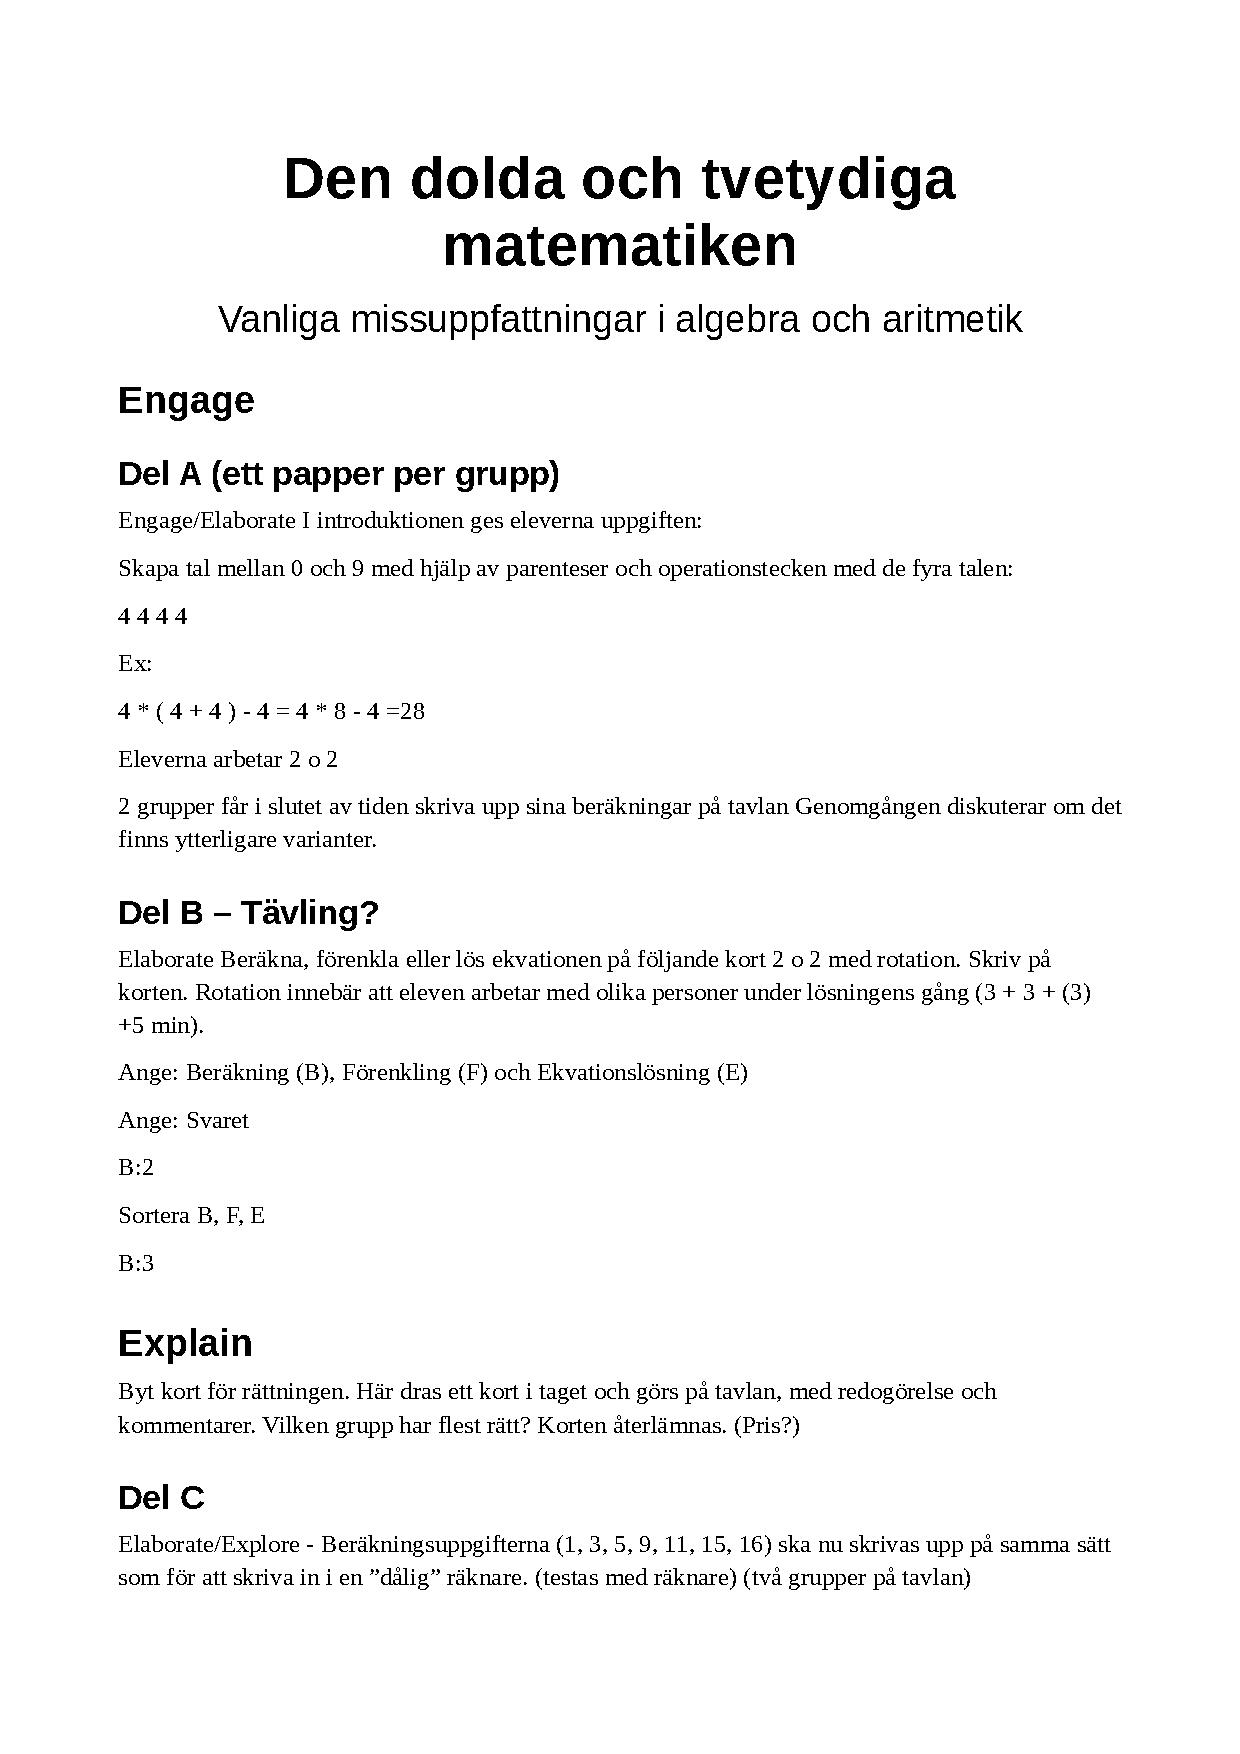
\includegraphics[page=1,width=1\textwidth]{pdf/tvetydig}}
\newpage
Teacher document page 2 of 4\\
\frame{\includegraphics[page=2,width=1\textwidth]{pdf/tvetydig}}
\newpage
Teacher document page 3 of 4\\
\frame{\includegraphics[page=3,width=1\textwidth]{pdf/tvetydig}}
\newpage
Teacher document page 4 of 4\\
\frame{\includegraphics[page=4,width=1\textwidth]{pdf/tvetydig}}